\documentclass[12pt,letterpaper]{article}

\usepackage[T1]{fontenc}
\usepackage[utf8]{inputenc}
\usepackage{lmodern}
\usepackage{microtype}
\usepackage{amsmath,amssymb,mathtools}
\usepackage{booktabs}
\usepackage{array}
\usepackage[margin=1in]{geometry}
\usepackage{graphicx}
\usepackage{setspace}
\usepackage[round,authoryear]{natbib}
\usepackage[hidelinks]{hyperref}
\usepackage{url}
\urlstyle{same}

\bibliographystyle{plainnat}

% ---------------------------------------------------------------------------
% Experiment numbers (auto-filled from Pipelines/11-Compare_Models.py output)
% ---------------------------------------------------------------------------
% Per-window metrics (mean $\pm$ std over test windows)
\newcommand{\rSimMean}{$0.0161 \pm 0.0063$}   \newcommand{\rCpxMean}{$0.0097 \pm 0.0044$}   \newcommand{\rDlpmMean}{$0.0025 \pm 0.0023$}
\newcommand{\rSimVol}{$0.0851 \pm 0.0930$}    \newcommand{\rCpxVol}{$0.1128 \pm 0.0657$}    \newcommand{\rDlpmVol}{$0.1255 \pm 0.1138$}
\newcommand{\rSimKurt}{$3.3318 \pm 4.4964$}   \newcommand{\rCpxKurt}{$7.0425 \pm 4.0269$}   \newcommand{\rDlpmKurt}{$3.3388 \pm 4.8726$}
\newcommand{\rSimKS}{$0.626 \pm 0.189$}     \newcommand{\rCpxKS}{$0.537 \pm 0.157$}     \newcommand{\rDlpmKS}{$0.252 \pm 0.103$}
\newcommand{\rSimKSp}{$0.010 \pm 0.054$}    \newcommand{\rCpxKSp}{$0.009 \pm 0.038$}    \newcommand{\rDlpmKSp}{$0.293 \pm 0.289$}
\newcommand{\rSimWD}{$0.0174 \pm 0.0056$}     \newcommand{\rCpxWD}{$0.0140 \pm 0.0044$}     \newcommand{\rDlpmWD}{$0.0062 \pm 0.0047$}
\newcommand{\rSimQQ}{$0.900 \pm 0.073$}     \newcommand{\rCpxQQ}{$0.742 \pm 0.114$}     \newcommand{\rDlpmQQ}{$0.915 \pm 0.074$}
% Pooled statistics
\newcommand{\poolKurtReal}{$9.48$} \newcommand{\poolKurtSim}{$3.19$} \newcommand{\poolKurtCpx}{$6.45$} \newcommand{\poolKurtDlpm}{$1.51$}
\newcommand{\poolSkewReal}{$0.63$} \newcommand{\poolSkewSim}{$-1.05$} \newcommand{\poolSkewCpx}{$-1.32$} \newcommand{\poolSkewDlpm}{$-0.13$}
\newcommand{\poolVolReal}{$0.256$}  \newcommand{\poolVolSim}{$0.234$}  \newcommand{\poolVolCpx}{$0.339$}  \newcommand{\poolVolDlpm}{$0.159$}
\newcommand{\poolQloReal}{$-0.0796$}  \newcommand{\poolQloSim}{$-0.0668$}  \newcommand{\poolQloCpx}{$-0.0955$}  \newcommand{\poolQloDlpm}{$-0.0383$}
\newcommand{\poolQhiReal}{$0.1057$}  \newcommand{\poolQhiSim}{$0.0489$}  \newcommand{\poolQhiCpx}{$0.0880$}  \newcommand{\poolQhiDlpm}{$0.0369$}
\newcommand{\poolAcfReal}{$0.213$}  \newcommand{\poolAcfSim}{$-0.124$}  \newcommand{\poolAcfCpx}{$-0.148$}  \newcommand{\poolAcfDlpm}{$0.029$}
\newcommand{\poolKSSim}{$0.463$}    \newcommand{\poolKSCpx}{$0.379$}   \newcommand{\poolKSDlpm}{$0.112$}
\newcommand{\poolWDSim}{$0.0129$}    \newcommand{\poolWDCpx}{$0.0099$}   \newcommand{\poolWDDlpm}{$0.0039$}
% DLIM ablation
\newcommand{\dlimKurt}{$168.39$} \newcommand{\dlimKS}{$0.102$} \newcommand{\dlimSpeedup}{10}
\newcommand{\nTestWindows}{400}
% Neural SDE baseline
\newcommand{\rSdeMean}{$0.0025 \pm 0.0029$}  \newcommand{\rSdeVol}{$0.0862 \pm 0.0808$} \newcommand{\rSdeKurt}{$3.1633 \pm 4.6684$}
\newcommand{\rSdeKS}{$0.202 \pm 0.086$}    \newcommand{\rSdeKSp}{$0.443 \pm 0.306$} \newcommand{\rSdeWD}{$0.0050 \pm 0.0037$}
\newcommand{\rSdeQQ}{$0.920 \pm 0.065$}    \newcommand{\poolKurtSde}{$2.90$}
\newcommand{\poolKSSde}{$0.031$} \newcommand{\poolAcfSde}{$0.049$}
% Chronos (TSFM) baseline
\newcommand{\rTsfmMean}{$0.0024 \pm 0.0026$}  \newcommand{\rTsfmVol}{$0.0937 \pm 0.0952$} \newcommand{\rTsfmKurt}{$3.4821 \pm 5.0333$}
\newcommand{\rTsfmKS}{$0.266 \pm 0.080$}    \newcommand{\rTsfmKSp}{$0.205 \pm 0.254$} \newcommand{\rTsfmWD}{$0.0056 \pm 0.0039$}
\newcommand{\rTsfmQQ}{$0.881 \pm 0.077$}    \newcommand{\poolKurtTsfm}{$12.93$}
\newcommand{\poolKSTsfm}{$0.172$} \newcommand{\poolAcfTsfm}{$0.026$}
\newcommand{\macroSdeDiscussion}{Table~\ref{tab:baselines} yields a nuanced
cross-family picture. The neural SDE, trained by exact stepwise maximum
likelihood, is the strongest marginal calibrator: it attains the lowest
per-window KS statistic and Wasserstein distance, as expected for an
objective that directly optimizes the conditional one-step density. Its
failure is structural, not statistical: with conditionally Gaussian
innovations its pooled excess kurtosis reaches only \poolKurtSde{} against
the market's \poolKurtReal{}, and volatility clustering (\poolAcfSde{})
falls far short of the real \poolAcfReal{}---no amount of training can
close a gap the model class forbids. Zero-shot Chronos is the mirror image:
pretraining scale buys it the most realistic \emph{unconditional} tail mass
(pooled kurtosis \poolKurtTsfm{}, extreme quantiles closest to the data),
but it consumes no contract features, its per-window shape metrics trail
the DLPM (KS \rTsfmKS{} versus \rDlpmKS{}; QQ $R^2$ \rTsfmQQ{} versus
\rDlpmQQ{}), its clustering is the weakest (\poolAcfTsfm{}), and its
250-step horizon lies well beyond the 64 steps the model is optimized for.
The DLPM sits between the two: within striking distance of the neural SDE
on every calibration metric while being the only conditional generator
whose noise mechanism can, in principle, express heavy tails---making
longer training, rather than architectural change, the natural route to
combining both strengths.}
% ---------------------------------------------------------------------------

% Table note environment (finance-journal style: notes below the table)
\newcommand{\tabnote}[1]{\begin{minipage}{\linewidth}\vspace{4pt}\footnotesize\singlespacing #1\end{minipage}}

\begin{document}

% ============================= TITLE PAGE ==================================
\begin{titlepage}
\begin{center}
\vspace*{1.2cm}
{\Large\bfseries Conditional Diffusion Models for Exotic Option Valuation:\\[4pt]
Heavy-Tailed Path Generation and Economic Value in a P--Q Game\par}

\vspace{1.4cm}
{\large Helin Zhao\footnote{Johns Hopkins University.}
\qquad
Junchi Shen\footnote{Johns Hopkins University. Corresponding author.}\par}

\vspace{0.8cm}
{This version: July 2026\par}
\end{center}

\vspace{1.2cm}
\begin{abstract}
\noindent
We study conditional denoising diffusion models as path generators for exotic
option valuation on Chinese equity indices. Holding a conditional U-Net
backbone fixed, we compare three generators: a Gaussian diffusion model
(DDPM) trained with a composite finance-aware loss, the same model trained
with the plain denoising loss, and a heavy-tailed Denoising L\'evy
Probabilistic Model (DLPM) driven by $\alpha$-stable noise and trained with
its standard loss. On held-out windows, the DLPM dominates both Gaussian
variants on distributional fidelity---halving the Kolmogorov--Smirnov
statistic and reducing Wasserstein distance and mean error severalfold---
while the composite loss, not the driving noise, governs pooled tail mass at
this training scale. Benchmarked further against a maximum-likelihood neural
SDE and a zero-shot time-series foundation model, the DLPM offers the
strongest balance of conditional shape fidelity among generators with a
heavy-tail mechanism. We further propose a P--Q dynamic game in which the
diffusion trader (P) quotes against a geometric Brownian motion market maker
(Q) across five product families. The P-model earns robust profits on
European and Asian options, while losses on lookbacks, accumulators, and
deep knock-in snowballs trace directly to the Gaussian generator's tail
underestimation. Replaying the game with matched-budget generators, the
DLPM converts the Gaussian model's deep knock-in snowball losses into large
stable profits with balanced positioning---distributional fidelity
monetizes precisely where tails dominate.
\end{abstract}

\vspace{0.6cm}
\noindent\textbf{Keywords:} exotic options; structured products; diffusion
models; L\'evy processes; $\alpha$-stable distributions; option pricing;
Monte Carlo simulation.

\medskip
\noindent\textbf{JEL classification:} G12; G13; C45; C53; C63.
\end{titlepage}
% ===========================================================================

\doublespacing

\section{Introduction}\label{sec:introduction}

Options and structured products provide contract holders with specific payoff
structures based on the performance of underlying assets at predetermined
times and conditions, and serve as effective tools for risk management,
hedging, and portfolio optimization. As financial markets have developed,
institutions have created a wide variety of exotic contracts: Asian, barrier,
lookback, and ratchet options add a single feature to vanilla options, while
snowball notes, phoenix notes, shark-fin options, and accumulators combine
multiple path-dependent conditions with intricate payoff structures
\citep{pesce2021exotic}.

Precisely because these products are diverse, customized, and structurally
complex, accurate pricing remains a core challenge for all market
participants. Buyers find it difficult to assess true value and risk; sellers
face significant losses from mispricing; regulators struggle to establish
unified evaluation mechanisms before risk exposures materialize. Accumulators
are a cautionary example: widely sold in Hong Kong and other Asian markets in
the 2000s, their path-dependent structure exposed extreme risks in volatile
periods, earning the market nickname ``I will kill you later.'' More
recently, in the 2024 Chinese A-share market, investors in snowball
autocallables suffered severe principal losses when market declines triggered
knock-in barriers, sparking intense public debate.

From the standpoint of practicality and versatility, simulation
methods---particularly Monte Carlo simulation \citep{boyle1977options}---remain
the most cost-effective approach to pricing path-dependent products: simulated
paths of the underlying, combined with the payoff structure, price virtually
any contract. Traditional Monte Carlo, however, rests on geometric Brownian
motion (GBM) dynamics with Gaussian increments, and therefore misses the
heavy tails, skewness, and volatility clustering that characterize real
returns \citep{cont2001empirical}. The consequences are not
academic: for barrier and knock-in products, tail probabilities are the
price.

Denoising diffusion models \citep{ho2020ddpm} approach path generation from
the opposite direction: a neural network learns to progressively restore the
data distribution from noise, generating market-style paths in reverse. Their
success in image and audio synthesis suggests they can capture the
distributional ``style'' of financial paths as well. Yet the classical DDPM
is itself driven by \emph{Gaussian} noise, so whether its paths can
reproduce extreme events is an open question that this paper examines
directly. The recently proposed Denoising L\'evy Probabilistic Model
\citep[DLPM;][]{shariatian2024dlpm} replaces Gaussian noise with heavy-tailed
$\alpha$-stable noise while retaining the computational skeleton of DDPM,
providing a principled heavy-tailed alternative.

This paper makes four contributions. First, we introduce conditional
denoising diffusion generators---both Gaussian and L\'evy-driven---to exotic
option valuation on Chinese equity indices, conditioning path generation on
contract-level features (initial price, historical volatility, risk-free
rate, tenor, and underlying identity). Second, we conduct a controlled
ablation that isolates the role of the training objective from that of the
driving noise: under one backbone and budget we compare (i) a composite
finance-aware loss regularizing volatility clustering, tails, drift,
quantiles, and the return spectrum; (ii) the plain denoising loss; and (iii)
the standard DLPM loss with $\alpha$-stable noise; two external
baselines---a maximum-likelihood neural SDE and a zero-shot time-series
foundation model---complete the comparison. The heavy-tailed model class
delivers the largest gain in conditional distributional fidelity, while
auxiliary loss engineering governs pooled tail mass at a fixed training
scale. Third, we propose a P--Q dynamic game that measures the
\emph{economic} value of generated paths: the diffusion-based trader (P)
quotes against a GBM Monte Carlo market maker (Q) across European, lookback,
Asian, accumulator, and snowball contracts. Fourth, we provide a reproducible
pipeline covering data construction, training, generation, statistical
evaluation, and adversarial backtesting.

We deliberately adopt the trader's (P-measure) perspective throughout;
risk-neutral calibration of the generator into a Q-pricing model is left to
future work. The remainder of the paper proceeds as follows.
Section~\ref{sec:literature} reviews related work.
Section~\ref{sec:data} describes the data.
Section~\ref{sec:method} presents the Gaussian and L\'evy diffusion
methodologies and the three training objectives.
Section~\ref{sec:experiments} reports the controlled generator ablation.
Section~\ref{sec:game} presents the P--Q game.
Section~\ref{sec:conclusion} concludes.

\section{Related Literature}\label{sec:literature}

\subsection{Pricing structured products and exotic options}

Industry practice relies on four methodologies \citep{deng2014valuation}:
simulation, which averages discounted payoffs over generated price paths and
suits strongly path-dependent products; numerical integration, when payoff
and density admit closed forms; decomposition into bonds, vanilla options,
and simpler exotics; and partial differential equation methods, which capture
continuous state dynamics at high solution cost. The Black--Scholes model,
despite its centrality for vanilla options, handles multi-layered structures
poorly given its risk-neutrality assumption and single volatility parameter.

A long literature refines these tools: Monte Carlo pricing from
\citet{boyle1977options}, jump-diffusion dynamics from
\citet{merton1976option}, Brownian-bridge quasi-Monte Carlo constructions
\citep{lin2008brownian}, ant colony optimization \citep{kumar2009aco}, and
tensor-network acceleration of lattice pricing \citep{vandamme2025tensor}.
Machine-learning approaches include LSTM option pricing
\citep{pimentel2025lstm}, generative adversarial models for arbitrage-free
implied volatility surfaces \citep{vuletic2025volgan}, and risk-neutral
pricing via GANs \citep{choi2025riskneutral}.

\subsection{Diffusion models for time series}

Denoising diffusion probabilistic models were established by
\citet{ho2020ddpm}, refined by the cosine schedule of
\citet{nichol2021improved}, and accelerated by the deterministic DDIM sampler
of \citet{song2020ddim}. TimeGrad \citep{rasul2021timegrad} pioneered
conditional diffusion for probabilistic time-series forecasting;
DiffSTOCK \citep{daiya2024diffstock} applies relational diffusion to equity
prediction; \citet{meijer2024rise} survey the area.

Diffusion models have recently become the leading generative approach for
financial time series. \citet{takahashi2025diffusion} show that denoising
diffusion models reproduce the stylized facts of asset
returns---heavy tails, volatility clustering, and dependence
structure---more faithfully than GANs and variational autoencoders, without
mode collapse; subsequent work extends the framework to conditional
multivariate generation with asset-specific and systematic covariates. Yet
the same literature emphasizes an open problem: no generator has fully
captured all stylized facts simultaneously, with tail behavior proving the
most stubborn. This gap motivates our heavy-tailed model class.

Classical diffusion is Gaussian-driven. For heavy-tailed data,
\citet{shariatian2024dlpm} propose the DLPM, which replaces Gaussian
increments with isotropic $\alpha$-stable noise, $\alpha \in (1,2]$
\citep{samorodnitsky1994stable}. Exploiting the variance-mixing
representation of stable laws, DLPM retains DDPM's computational structure
with minimal changes while markedly improving tail coverage; $\alpha = 2$
recovers the Gaussian DDPM exactly. Given the well-documented heavy tails of
asset returns \citep{cont2001empirical}, DLPM is a natural generator for
financial paths; to our knowledge this paper is the first to evaluate it in a
derivatives-valuation setting.

\subsection{Alternative model families}

Two further families compete in this space. \emph{Neural stochastic
differential equations} parameterize the drift and diffusion of an SDE by
neural networks, trained by likelihood or adversarial criteria
\citep{gierjatowicz2020neural}; imposing no-arbitrage constraints yields
market models suitable for risk-neutral applications
\citep{cohen2023neuralsde}. \emph{Time-series foundation models} such as
Chronos \citep{ansari2024chronos} and TimesFM \citep{das2024timesfm} are
transformers pretrained on billions of observations that produce zero-shot
probabilistic forecasts; however, generic foundation models tend to
underperform domain-specific architectures on financial data, and their
uncertainty calibration remains an open concern. Because both families are
natural alternatives to diffusion generators, our empirical study includes a
conditional neural-SDE baseline trained on identical data
(Section~\ref{sec:baselines}), positioning the diffusion results against the
classical SDE paradigm rather than against Gaussian Monte Carlo alone.

\section{Data}\label{sec:data}

\subsection{Sample construction}

Our underlying universe consists of broad Chinese equity indices. The
CSI~1000---covering small- and mid-cap names---is a common underlying for
over-the-counter options and snowball structures; we augment it with the
CSI~300, CSI~500, and SSE Composite to form the pooled training universe.
Daily index data from January 1, 2014 to August 1, 2025 are obtained via
\texttt{akshare}. For the risk-free rate we follow OTC market-maker practice
and use SHIBOR, matched to each contract's tenor from observed maturities
$M \in \{30, 60, 90, 180, 365\}$ calendar days, front-filled by date.

We employ sliding windows of 30, 90, 180, and 365 calendar days,
corresponding to 1-, 3-, 6-, and 12-month risk-free tenors, sliced daily to
produce historical price-path samples. The sample is split into training and
out-of-sample test sets at January 1, 2024, with strict look-ahead
prevention on both sides: every training window's realized path terminates
by December 3, 2023, so no training path overlaps the test period, and an
embargo of roughly one month separates the last training observation from
the first test window (January 2, 2024). Because windows slide daily, both
sets contain overlapping observations; all reported statistics should be
read accordingly, as the effective number of independent observations is
smaller than the window count. The single-index CSI~1000 subsample used in the P--Q game
contains 8{,}023 training and 827 test paths; the pooled Chinese-index sample
used in the generator ablation contains 32{,}092 training windows.

\subsection{Variable definitions and preprocessing}

Let $C$ denote calendar days and $T \subset C$ trading days. For
$s, t \in C$, $CD(s,t)$ counts calendar days from $s$ (inclusive) to $t$
(exclusive) and $TD(s,t)$ counts trading days, so $TD(s,t) \le CD(s,t)$.
Calendar and trading times to maturity are $T_{\mathrm{cal}} = CD(s,T)/365$
and $T_{\mathrm{trad}} = TD(s,T)/252$. With $S_t$ the index level on trading
days, daily log returns are $r_t = \ln(S_t / S_{t-1})$, and for a window of
$n$ returns the sample mean and volatility are
\begin{equation}
\bar r = \frac{1}{n}\sum_{t=1}^{n} r_t,
\qquad
\sigma_{\mathrm{daily}} = \sqrt{\frac{1}{n-1}\sum_{t=1}^{n}(r_t - \bar r)^2},
\qquad
\sigma_{\mathrm{ann}} = \sigma_{\mathrm{daily}}\sqrt{252}.
\end{equation}

Each path is transformed to scaled log-return space,
$x_{0,k} = r_k / s_{\mathrm{vol}}$ with $s_{\mathrm{vol}} = 0.09$, so that
paths are reconstructed from the initial price by exponentiating cumulative
returns. Windows shorter than the maximum length of 252 trading days are
zero-padded with a validity mask $M \in \{0,1\}^{B\times L}$
($M_{b,l} = 1$ for valid observations); all losses and statistics are
computed on valid positions only:
\begin{equation}
L_{\mathrm{masked}} = \frac{1}{\sum_{b,l} M_{b,l}}
\sum_{b=1}^{B}\sum_{l=1}^{L} M_{b,l}\,\bigl(y_{b,l} - \hat y_{b,l}\bigr)^2 .
\label{eq:maskedmse}
\end{equation}

Each window carries a condition vector
$c = (\tilde S_0, \sigma_{\mathrm{hist}}, r_f, T_{\mathrm{cal}},
\rho_{\mathrm{trad}}, \mathrm{id}_{\mathrm{country}},
\mathrm{id}_{\mathrm{index}})$: five standardized numerical features
(normalized initial price, trailing one-year volatility, matched risk-free
rate, calendar tenor, and the ratio of trading to calendar days) plus two
categorical identifiers embedded by the network
(Appendix~\ref{app:architecture}).

\section{Methodology}\label{sec:method}

\subsection{Gaussian conditional diffusion}\label{sec:ddpm}

The forward process of a DDPM is a Markov chain that gradually corrupts the
data $x_0 \in \mathbb{R}^{B \times C \times L}$ with Gaussian noise,
\begin{equation}
q(x_t \mid x_{t-1}) = \mathcal{N}\bigl(x_t;\ \sqrt{1-\beta_t}\,x_{t-1},\
\beta_t I\bigr),
\end{equation}
under the cosine schedule $\beta_t$ of \citet{nichol2021improved} with
$T = 500$ steps. With $\alpha_t = 1 - \beta_t$ and
$\bar\alpha_t = \prod_{i \le t} \alpha_i$, the marginal admits the
reparameterization
\begin{equation}
x_t = \sqrt{\bar\alpha_t}\,x_0 + \sqrt{1-\bar\alpha_t}\,\epsilon_t,
\qquad \epsilon_t \sim \mathcal{N}(0, I).
\end{equation}

The reverse process approximates $q(x_{t-1} \mid x_t, x_0)$ by a Gaussian
transition conditioned on contract features $c$,
\begin{equation}
p_\theta(x_{t-1} \mid x_t, c) = \mathcal{N}\bigl(x_{t-1};\
\mu_\theta(x_t, t, c),\ \tilde\beta_t I\bigr),
\end{equation}
where the conditional U-Net (Appendix~\ref{app:architecture}) outputs
$\hat x_0 = f_\theta(x_t, t, c)$ and the posterior mean and variance follow
from Bayes' rule for the Gaussian chain:
\begin{equation}
\tilde\mu_t(x_t, \hat x_0)
= \frac{\sqrt{\bar\alpha_{t-1}}\,\beta_t}{1-\bar\alpha_t}\,\hat x_0
+ \frac{\sqrt{\alpha_t}\,(1-\bar\alpha_{t-1})}{1-\bar\alpha_t}\,x_t,
\qquad
\tilde\beta_t = \frac{1-\bar\alpha_{t-1}}{1-\bar\alpha_t}\,\beta_t .
\end{equation}

For fast generation we use the deterministic DDIM sampler
\citep{song2020ddim}: for a subsequence $\{\tau_i\} \subset \{1,\dots,T\}$,
\begin{equation}
x_{\tau_{i-1}}
= \sqrt{\bar\alpha_{\tau_{i-1}}}\,
\underbrace{\frac{x_{\tau_i} - \sqrt{1-\bar\alpha_{\tau_i}}\,
\hat\epsilon_{\tau_i}}{\sqrt{\bar\alpha_{\tau_i}}}}_{\hat x_0}
+ \sqrt{1-\bar\alpha_{\tau_{i-1}} - \sigma_{\tau_i}^2}\;\hat\epsilon_{\tau_i}
+ \sigma_{\tau_i}\, z,
\qquad z \sim \mathcal{N}(0, I),
\end{equation}
with $\sigma_{\tau_i} = 0$ in the fully deterministic case.

\subsection{Training objective I: simple loss}\label{sec:simpleloss}

The \emph{simple} objective is the standard masked denoising regression of
Eq.~\eqref{eq:maskedmse} applied to the network's clean-sequence prediction:
\begin{equation}
\mathcal{L}_{\mathrm{simple}}
= \mathbb{E}_{t,\,x_0,\,\epsilon}
\Bigl[\bigl\| M \odot \bigl(f_\theta(x_t, t, c) - x_0\bigr) \bigr\|_2^2
\big/ \textstyle\sum M \Bigr].
\label{eq:simple}
\end{equation}
This is the direct analogue of the original DDPM objective and embeds no
financial domain knowledge.

\subsection{Training objective II: composite finance-aware loss}\label{sec:complexloss}

Financial returns exhibit stylized facts---volatility clustering, heavy
tails, skewness, and characteristic spectra---that pure mean-squared error
does not explicitly reward \citep{cont2001empirical}. The \emph{composite}
objective augments Eq.~\eqref{eq:simple} with auxiliary regularizers
computed between the predicted clean sequence $\hat x_0$ and the target
$x_0$, all masked as in Eq.~\eqref{eq:maskedmse}:
\begin{align}
L_{\mathrm{jump}} &= \bigl\| (\hat x_{0,i+1} - \hat x_{0,i}) -
(x_{0,i+1} - x_{0,i}) \bigr\|_1
&& \text{(relative jumps)}, \\
L_{\mathrm{vol}} &= \mathrm{SmoothL1}\bigl(\mathrm{Std}(\hat
x_{0,\mathrm{win}}),\ \mathrm{Std}(x_{0,\mathrm{win}})\bigr)
&& \text{(volatility clustering)}, \\
L_{\mathrm{gvol}} &= \bigl|\sigma_{\mathrm{pred}} -
\sigma_{\mathrm{true}}\bigr|
&& \text{(global volatility)}, \\
L_{\mathrm{kurt}} &= \bigl(K_{\mathrm{pred}} - K_{\mathrm{true}}\bigr)^2,
\quad K = \mathbb{E}[z^4] - 3
&& \text{(heavy tails)}, \\
L_{\mathrm{skew}} &= \bigl(\mathbb{E}[z_{\mathrm{pred}}^3] -
\mathbb{E}[z_{\mathrm{true}}^3]\bigr)^2
&& \text{(skewness)}, \\
L_{\mathrm{drift}} &= \Bigl(\textstyle\sum_i \Delta\hat x_{0,i} -
\sum_i \Delta x_{0,i}\Bigr)^2
&& \text{(terminal drift)}, \\
L_{\mathrm{quant}} &= \textstyle\sum_{\tau \in \{0.01, 0.99\}}
L_\tau\bigl(q_\tau(x_0),\ q_\tau(\hat x_0)\bigr)
&& \text{(extreme quantiles)}, \\
L_{\mathrm{spec}} &= \mathrm{SmoothL1}\bigl(\hat P_{\mathrm{norm}},\
P_{\mathrm{norm}}\bigr)
&& \text{(power spectrum)},
\end{align}
where $z$ denotes the standardized sequence, $L_\tau$ is the pinball loss of
\citet{wang2019pinball} at quantile $\tau$, and
$P_{\mathrm{norm}}[k] = P[k]/\max_k P[k]$ is the normalized discrete Fourier
magnitude spectrum. The extreme-quantile pair $\tau \in \{0.01, 0.99\}$
penalizes underestimation of both tails asymmetrically, sharpening the
delineation of downside risk and upside potential.

Because the auxiliary terms live on heterogeneous scales, each is normalized
by an exponential moving average (EMA) of its own magnitude, and all
auxiliary weights are annealed linearly from zero over a warm-up phase
($s = \min(1, \mathrm{step}/\mathrm{warmup})$):
\begin{equation}
\mathcal{L}_{\mathrm{complex}}
= \mathcal{L}_{\mathrm{simple}}
+ s \sum_{k \in \mathcal{K}} \lambda_k\,
\frac{L_k}{\mathrm{EMA}[L_k] + \varepsilon},
\label{eq:complex}
\end{equation}
with base weights
$(\lambda_{\mathrm{jump}}, \lambda_{\mathrm{vol}}, \lambda_{\mathrm{gvol}},
\lambda_{\mathrm{kurt}}, \lambda_{\mathrm{skew}}, \lambda_{\mathrm{drift}},
\lambda_{\mathrm{quant}}, \lambda_{\mathrm{spec}})
= (0.5, 3.5, 8, 5, 0.5, 2, 3, 2)$.

\subsection{Heavy-tailed diffusion: the DLPM}\label{sec:dlpm}

Gaussian diffusion imposes light-tailed increments on the forward chain. The
DLPM of \citet{shariatian2024dlpm} replaces them with isotropic
$\alpha$-stable noise, yielding a generator whose prior and reverse dynamics
are heavy-tailed by construction. Let
$\varepsilon^{(\alpha)} \sim \mathcal{S}\alpha\mathcal{S}(I)$ denote
isotropic symmetric $\alpha$-stable noise with stability index
$\alpha \in (1, 2]$; $\alpha = 2$ recovers the Gaussian case. The forward
chain is
\begin{equation}
x_t = \gamma_t\, x_{t-1} + \sigma_t\, \varepsilon_t^{(\alpha)},
\qquad t = 1, \dots, T,
\end{equation}
under a \emph{scale-preserving} schedule: with
$\bar\gamma_t = \prod_{i\le t}\gamma_i$, the stability property gives the
marginal
\begin{equation}
x_t = \bar\gamma_t\, x_0 + \bar\sigma_t\, \bar\varepsilon^{(\alpha)},
\qquad
\bar\sigma_t = \bigl(1 - \bar\gamma_t^{\,\alpha}\bigr)^{1/\alpha},
\end{equation}
so $\bar\gamma_t^{\,\alpha} + \bar\sigma_t^{\,\alpha} = 1$ generalizes
variance preservation. We derive $\gamma_t = \alpha_t^{1/\alpha}$ from the
same cosine schedule as the Gaussian model, so both models traverse
comparable signal-to-noise trajectories.

Computations with stable laws become Gaussian conditionally on an auxiliary
variable \citep{samorodnitsky1994stable}: any isotropic $\alpha$-stable
vector admits the \emph{variance-mixing} representation
\begin{equation}
\varepsilon^{(\alpha)} \overset{d}{=} \sqrt{a}\; Z,
\qquad
a \sim \mathcal{S}_{\alpha/2}^{+},\quad Z \sim \mathcal{N}(0, I),
\label{eq:mixing}
\end{equation}
with $\mathcal{S}_{\alpha/2}^{+}$ the totally skewed positive
$(\alpha/2)$-stable law. Conditionally on the chain $A = (a_1,\dots,a_T)$,
the forward process is Gaussian with stochastic variances and the reverse
conditional $q(x_{t-1}\mid x_t, x_0, A)$ is Gaussian with
\begin{equation}
\Sigma_t = \sigma_t^2\, a_t + \gamma_t^2\, \Sigma_{t-1},
\quad
\Gamma_t = 1 - \frac{\gamma_t^2\,\Sigma_{t-1}}{\Sigma_t},
\quad
\tilde m_{t-1} = \frac{x_t - \bar\sigma_t\,\Gamma_t\,\varepsilon_t}{\gamma_t},
\quad
\tilde\Sigma_{t-1} = \Gamma_t\, \Sigma_{t-1}.
\label{eq:posterior}
\end{equation}

\paragraph{Training objective III: standard DLPM loss.}
The network predicts the chain noise
$\varepsilon_t = (x_t - \bar\gamma_t x_0)/\bar\sigma_t$. A training sample is
constructed via Eq.~\eqref{eq:mixing},
\begin{equation}
a_t \sim \mathcal{S}_{\alpha/2}^{+}, \quad z \sim \mathcal{N}(0, I), \quad
x_t = \bar\gamma_t\, x_0 + \bar\sigma_t \sqrt{a_t}\, z,
\qquad \varepsilon_t = \sqrt{a_t}\, z,
\end{equation}
and the \emph{standard loss} is the $L_p$ objective
\begin{equation}
\mathcal{L}_{\mathrm{DLPM}}
= \mathbb{E}_{t,\,x_0,\,a_t,\,z}
\Bigl[\bigl\| M \odot \bigl(\hat\varepsilon_\theta(x_t, t, c) -
\varepsilon_t\bigr)\bigr\|_p \Bigr].
\label{eq:dlpmloss}
\end{equation}
Because $\alpha$-stable noise has infinite variance for $\alpha < 2$, the
exponent must respect a moment constraint; we use the \emph{unsquared} $L_2$
norm---an order-one moment of
$\|\varepsilon\|_2 = \sqrt{a}\,\|Z\|_2$---which is finite for all
$\alpha > 1$. \citet{shariatian2024dlpm} additionally propose a
median-of-means estimator over multiple draws of $a_t$; the single-draw
estimator proved sufficient at our scale. For numerical stability, extreme
draws of $a_t$ are clamped at $a_{\max} = 100$, affecting only the far tail
of the auxiliary variable. No financial regularizers of
Section~\ref{sec:complexloss} are applied: Eq.~\eqref{eq:dlpmloss} is exactly
the objective prescribed by the paper.

\paragraph{Sampling.}
\emph{Ancestral} sampling draws the auxiliary chain $A$ and initial noise
$x_T = \bar\sigma_T \varepsilon^{(\alpha)}$, then iterates the Gaussian
posterior of Eq.~\eqref{eq:posterior} with
$\varepsilon_t \to \hat\varepsilon_\theta(x_t, t, c)$. Because the variances
$\Sigma_t$ are driven by heavy-tailed $a_t$, individual reverse trajectories
can take occasional large steps---precisely the mechanism that reproduces
jumps. \emph{DLIM}, the deterministic skip-step analogue of DDIM, transports
the state exactly between noise levels of a subsequence $\{\tau_i\}$:
\begin{equation}
x_{\tau_{i-1}}
= \frac{\bar\gamma_{\tau_{i-1}}}{\bar\gamma_{\tau_i}}
\bigl(x_{\tau_i} - \bar\sigma_{\tau_i}\,\hat\varepsilon_{\tau_i}\bigr)
+ \bar\sigma_{\tau_{i-1}}\, \hat\varepsilon_{\tau_i}.
\label{eq:dlim}
\end{equation}

\section{Controlled Generator Ablation}\label{sec:experiments}

\subsection{Design}

All three variants share an identical conditional U-Net backbone (17.0
million parameters; Appendix~\ref{app:architecture}) and an identical
training budget, so the only varying factors are the driving noise and the
training objective:
\begin{description}
\item[DDPM-simple:] Gaussian diffusion, $x_0$-parameterization, simple
  masked denoising loss, Eq.~\eqref{eq:simple}.
\item[DDPM-complex:] identical Gaussian diffusion, composite finance-aware
  loss, Eq.~\eqref{eq:complex}.
\item[DLPM:] $\alpha$-stable diffusion with $\alpha = 1.8$,
  $\varepsilon$-parameterization, standard DLPM loss,
  Eq.~\eqref{eq:dlpmloss}.
\end{description}
Each model trains for 4{,}000 optimizer steps at batch size 64 (Adam,
learning rate $10^{-4}$ with cosine decay, EMA weight averaging with decay
0.995) on the 32{,}092 pooled Chinese-index windows with $T = 500$ diffusion
steps (Appendix~\ref{app:hyper}). Evaluation uses EMA weights and full-chain
ancestral sampling on \nTestWindows{} held-out post-2024 test windows: for
each window the model generates one path conditioned on that window's
contract features and validity mask, and per-window statistics compare
generated and realized scaled log returns.

\subsection{Path-level results}

Table~\ref{tab:persample} reports per-window statistics;
Table~\ref{tab:pooled} reports statistics of the pooled return
distributions.

\begin{table}[ht]
\singlespacing
\centering
\caption{Per-window generation quality on held-out test windows}
\label{tab:persample}
\begin{tabular}{lccc}
\toprule
Metric & DDPM-simple & DDPM-complex & DLPM ($\alpha{=}1.8$) \\
\midrule
Mean difference        & \rSimMean & \rCpxMean & \rDlpmMean \\
Volatility difference  & \rSimVol  & \rCpxVol  & \rDlpmVol  \\
Kurtosis difference    & \rSimKurt & \rCpxKurt & \rDlpmKurt \\
KS statistic           & \rSimKS   & \rCpxKS   & \rDlpmKS   \\
KS $p$-value           & \rSimKSp  & \rCpxKSp  & \rDlpmKSp  \\
Wasserstein distance   & \rSimWD   & \rCpxWD   & \rDlpmWD   \\
QQ $R^2$               & \rSimQQ   & \rCpxQQ   & \rDlpmQQ   \\
\bottomrule
\end{tabular}
\tabnote{This table reports the mean $\pm$ standard deviation, across
\nTestWindows{} held-out post-2024 test windows, of per-window discrepancies
between one generated path and the realized path sharing the same contract
conditions. Mean and volatility differences are absolute differences of the
return mean and annualized return volatility; the kurtosis difference is the
absolute difference of excess kurtosis; KS is the two-sample
Kolmogorov--Smirnov statistic; QQ $R^2$ is the coefficient of determination
of a linear fit through the paired empirical percentiles (1--99). Lower is
better except the KS $p$-value and QQ $R^2$. All models share the same U-Net
backbone, training budget, and sampling protocol.}
\end{table}

\begin{table}[ht]
\singlespacing
\centering
\caption{Pooled return-distribution statistics}
\label{tab:pooled}
\begin{tabular}{lcccc}
\toprule
Statistic & Real & DDPM-simple & DDPM-complex & DLPM \\
\midrule
Excess kurtosis            & \poolKurtReal & \poolKurtSim & \poolKurtCpx & \poolKurtDlpm \\
Skewness                   & \poolSkewReal & \poolSkewSim & \poolSkewCpx & \poolSkewDlpm \\
Annualized volatility      & \poolVolReal  & \poolVolSim  & \poolVolCpx  & \poolVolDlpm  \\
$0.1\%$ quantile           & \poolQloReal  & \poolQloSim  & \poolQloCpx  & \poolQloDlpm  \\
$99.9\%$ quantile          & \poolQhiReal  & \poolQhiSim  & \poolQhiCpx  & \poolQhiDlpm  \\
$|r|$ autocorrelation (lag 1) & \poolAcfReal & \poolAcfSim & \poolAcfCpx & \poolAcfDlpm \\
\midrule
Pooled KS vs.\ real        & --            & \poolKSSim   & \poolKSCpx   & \poolKSDlpm   \\
Pooled Wasserstein         & --            & \poolWDSim   & \poolWDCpx   & \poolWDDlpm   \\
\bottomrule
\end{tabular}
\tabnote{This table pools daily log returns across all test windows (real
column) and across the corresponding generated paths (model columns).
Quantiles are of the pooled daily log-return distribution; the $|r|$
autocorrelation is the average lag-one autocorrelation of absolute returns
within each window (a volatility-clustering proxy); the last two rows give
the distance between the pooled generated and pooled real distributions.}
\end{table}

\IfFileExists{figures/tail_density.png}{%
\begin{figure}[ht]
\singlespacing
\centering
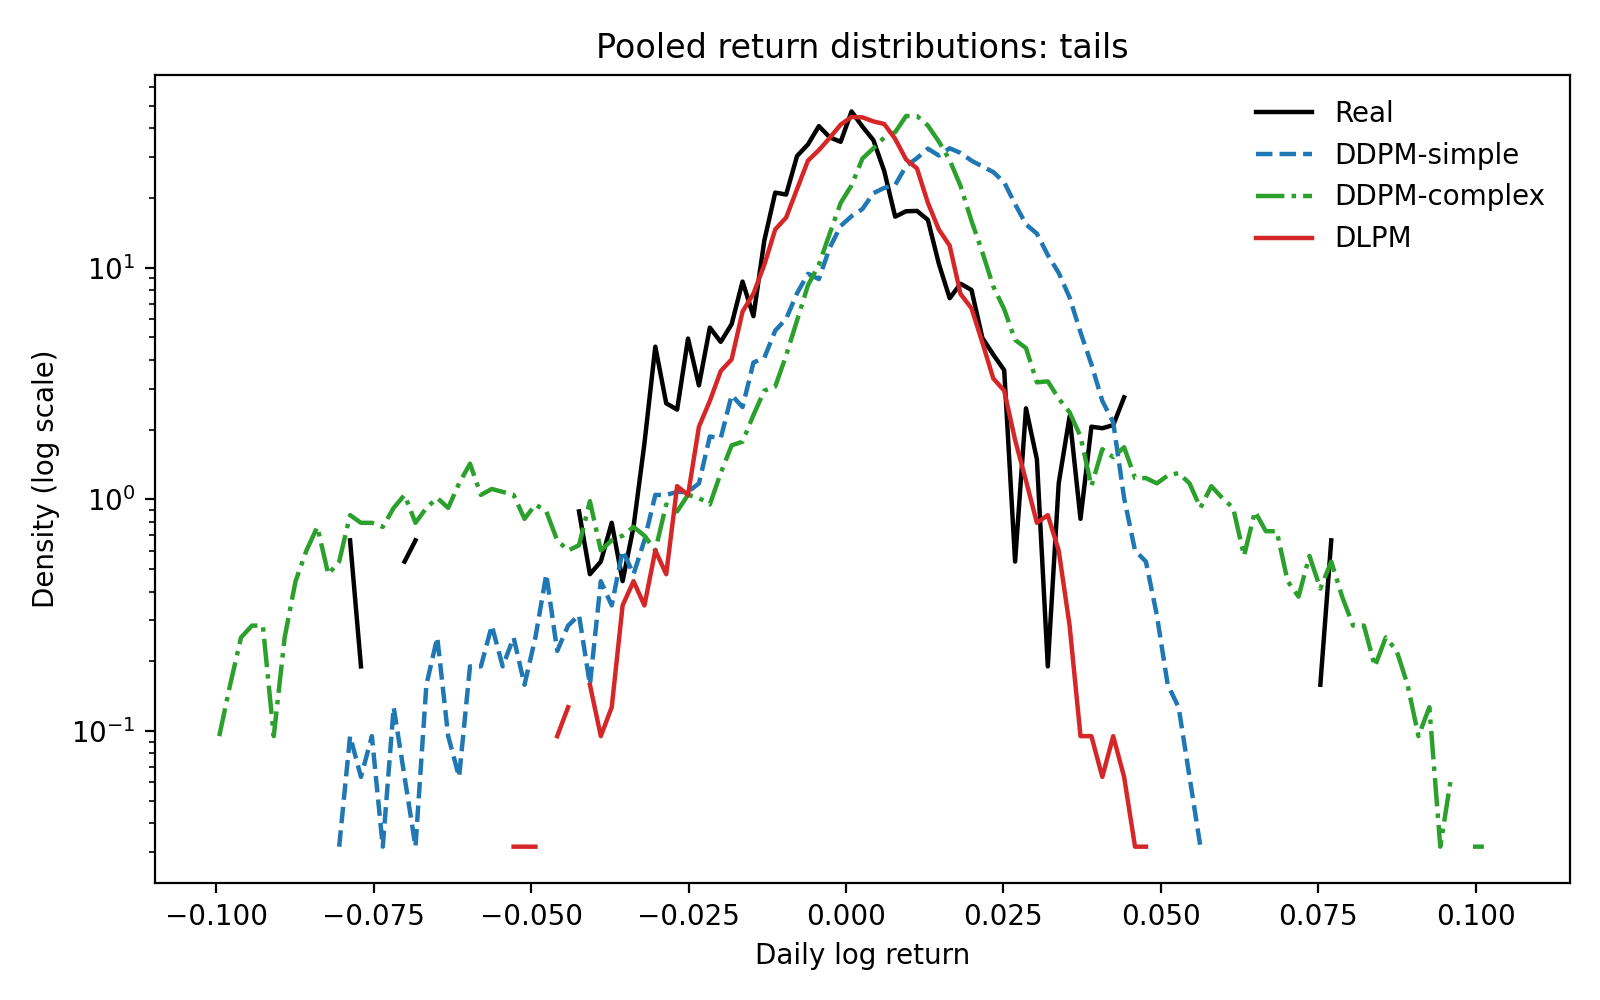
\includegraphics[width=0.82\textwidth]{figures/tail_density.png}
\caption{Pooled daily log-return densities (log scale). The figure overlays
the pooled return distribution of the realized test paths (Real) with those
of paths generated by the three model variants under identical conditions.
Distance from the real curve in the far tails visualizes each generator's
tail fidelity.}
\label{fig:tails}
\end{figure}
}{}

Three findings stand out. First, the DLPM with the plain paper-standard
loss dominates both Gaussian variants on every distribution-shape metric:
it halves the per-window KS statistic (\rDlpmKS{} versus \rSimKS{} and
\rCpxKS{}), is the only diffusion variant whose paths pass the KS test on
average (mean $p$-value \rDlpmKSp{} against $\approx 0.01$ for both
Gaussian variants), reduces the Wasserstein distance roughly threefold, and
attains the best mean alignment and QQ $R^2$. Second, the composite loss
shapes the Gaussian model exactly as designed but at a price: it pushes the
\emph{pooled} excess kurtosis to \poolKurtCpx{}---by far the closest to the
real \poolKurtReal{} among all trained models---yet degrades per-window
shape (kurtosis overshoot of \rCpxKurt{}, QQ $R^2$ falling to \rCpxQQ{}),
indicating that global tail regularizers inflate extremes indiscriminately
rather than matching conditional distributions. Third, at the fixed
4{,}000-step budget the DLPM's pooled kurtosis (\poolKurtDlpm{}) remains
far below the market's: the $\alpha$-stable mechanism is necessary but not
sufficient, because the bounded $\varepsilon$-head (a $\tanh$ output cap)
and the short schedule limit how much tail mass the trained network
expresses. Volatility clustering is weak across all variants, confirming
that clustering must be carried by the conditional backbone rather than by
the driving noise.

\subsection{Comparison with alternative model families}\label{sec:baselines}

To position the diffusion generators against competing paradigms, we
evaluate two additional baselines under the identical protocol. First, a
\emph{conditional neural SDE} \citep{gierjatowicz2020neural} trained on
identical data: daily log-price increments follow
$dX = \mu_\theta(h_t, c)\,dt + \sigma_\theta(h_t, c)\,dW_t$ under an
Euler--Maruyama discretization, where a recurrent state $h_t$ encodes the
realized return history, the contract features $c$ enter through an
embedding, and the drift and diffusion heads are trained by exact Gaussian
maximum likelihood with the same masking protocol. The model nests deep
stochastic-volatility dynamics: the recurrent state lets conditional
volatility respond to past returns (clustering), while innovations remain
conditionally Gaussian---precisely the property the DLPM relaxes. Second, a
\emph{time-series foundation model}: the pretrained Chronos-T5-small
\citep{ansari2024chronos} in zero-shot mode, which receives the yearlong
daily price history preceding each window's start date as context and
autoregressively samples a continuation of the window's length; sampled
levels are converted to log returns and scored identically. Unlike the
other models, Chronos consumes raw price history rather than contract
features, so its comparison probes what pretraining scale alone buys
without domain adaptation. Its pretraining corpus predates our 2024--2025
test period and is dominated by non-financial series, so the zero-shot
evaluation is free of look-ahead contamination.

\begin{table}[ht]
\singlespacing
\centering
\caption{Alternative model families versus diffusion generators}
\label{tab:baselines}
\begin{tabular}{lcccc}
\toprule
Metric & Neural SDE & Chronos & DDPM-complex & DLPM ($\alpha{=}1.8$) \\
\midrule
Mean difference        & \rSdeMean & \rTsfmMean & \rCpxMean & \rDlpmMean \\
Volatility difference  & \rSdeVol  & \rTsfmVol  & \rCpxVol  & \rDlpmVol  \\
Kurtosis difference    & \rSdeKurt & \rTsfmKurt & \rCpxKurt & \rDlpmKurt \\
KS statistic           & \rSdeKS   & \rTsfmKS   & \rCpxKS   & \rDlpmKS   \\
KS $p$-value           & \rSdeKSp  & \rTsfmKSp  & \rCpxKSp  & \rDlpmKSp  \\
Wasserstein distance   & \rSdeWD   & \rTsfmWD   & \rCpxWD   & \rDlpmWD   \\
QQ $R^2$               & \rSdeQQ   & \rTsfmQQ   & \rCpxQQ   & \rDlpmQQ   \\
\midrule
Pooled excess kurtosis (real: \poolKurtReal) & \poolKurtSde & \poolKurtTsfm & \poolKurtCpx & \poolKurtDlpm \\
Pooled KS vs.\ real    & \poolKSSde   & \poolKSTsfm   & \poolKSCpx   & \poolKSDlpm   \\
$|r|$ autocorrelation (real: \poolAcfReal) & \poolAcfSde & \poolAcfTsfm & \poolAcfCpx & \poolAcfDlpm \\
\bottomrule
\end{tabular}
\tabnote{The neural SDE parameterizes drift and diffusion of daily
log-price increments by neural networks with a recurrent state and is
trained by Gaussian maximum likelihood on the same training windows,
conditions, and masks as the diffusion models. Chronos-T5-small
\citep{ansari2024chronos} is evaluated zero-shot: for each test window it
receives the preceding (up to) 252 trading-day price history of the same
index as context and samples one continuation of the window's length.
Evaluation follows the protocol of Table~\ref{tab:persample} on the same
\nTestWindows{} test windows. Definitions as in
Tables~\ref{tab:persample} and~\ref{tab:pooled}.}
\end{table}

\macroSdeDiscussion{}

\subsection{Accelerated sampling}

Replacing the 500-step ancestral chain by 50-step deterministic DLIM
(Eq.~\ref{eq:dlim}) reduces sampling time by a factor of roughly
\dlimSpeedup{} and leaves the calibration metrics essentially
unchanged---the pooled KS statistic even improves slightly to \dlimKS{}.
The caveat is at the extremes: with only 50 large steps, occasional windows
saturate the sampler's stability bounds, inflating the pooled excess
kurtosis to \dlimKurt{}. We therefore recommend DLIM for
calibration-sensitive workloads (fast valuation loops such as the game of
Section~\ref{sec:game}) and the full ancestral chain for tail-sensitive
risk applications.

\subsection{Static validation of the production P-model}

Independently of the controlled ablation, the production DDPM-complex
P-model used in the P--Q game (trained to full convergence on the CSI~1000
subsample) was validated statically on its 827-window test set
(Table~\ref{tab:static}).

\begin{table}[ht]
\singlespacing
\centering
\caption{Static validation of the production P-model (CSI~1000)}
\label{tab:static}
\begin{tabular}{lcc}
\toprule
 & Mean & Std \\
\midrule
Mean difference       & 0.0053  & 0.0037 \\
Volatility difference & 0.1137  & 0.0922 \\
Kurtosis difference   & 3.559   & 3.517  \\
KS statistic          & 0.199   & 0.094  \\
KS $p$-value          & 0.2087  & 0.2407 \\
Wasserstein distance  & 0.00836 & 0.00505 \\
QQ $R^2$              & 0.889   & 0.0518 \\
\bottomrule
\end{tabular}
\tabnote{Definitions as in Table~\ref{tab:persample}, computed on the 827
held-out CSI~1000 windows used in the P--Q game of Section~\ref{sec:game}.}
\end{table}

The production model excels at the core statistics: the mean difference is
0.0053, the Wasserstein distance is small, and the average KS $p$-value of
0.2087 means equality of distributions cannot be rejected at the 5\% level;
the QQ $R^2$ of 0.889 confirms strong quantile correspondence. The single
glaring weakness is the kurtosis difference of 3.56---by far the largest
discrepancy: Gaussian-diffusion tails remain ``thinner'' than the market's
even though the training loss explicitly penalizes kurtosis mismatch. This
diagnosis is what motivates the heavy-tailed DLPM studied in the controlled
ablation above, whose noise mechanism removes the structural obstacle even
though fully expressing market-level kurtosis requires training beyond the
ablation budget.

\section{The Trader--Market-Maker Dynamic Quoting Game}\label{sec:game}

As a P-measure model, the diffusion generator naturally invites expectations
about out-of-sample trading performance. We therefore pair the P-model
against a risk-neutral Q-model acting as counterparty in backtests over the
827 CSI~1000 test windows.

\subsection{Game framework}

The Q side is a GBM Monte Carlo pricer. This choice serves two purposes:
P and Q receive identical inputs, enabling clean head-to-head comparisons,
and GBM Monte Carlo remains the canonical risk-neutral pricing approach. To
mitigate the limitations of the baseline Q pricer, we evaluate the market
maker under varying profit targets (a \emph{greediness} parameter $g$): when
selling, Q quotes $(1+g)$ times its risk-neutral price; when buying, it
accepts $(1-g)$ times that price, giving it margin to profit after hedging
even under model error. A trade executes only when the relative P--Q price
gap exceeds 10\%, a threshold intended to cover transaction costs and filter
weak signals. For snowball notes, whose value is dominated by coupon terms,
greediness is instead an absolute spread $\Delta$ on the note value. Because
test windows slide daily, consecutive trades reference largely overlapping
price paths; cumulative P\&L therefore aggregates dependent positions, and
Sharpe ratios computed from these trades overstate risk-adjusted
performance relative to independent bets.

\subsection{Product set}

We consider five contract families. \emph{European options}
($K = S_0$) evaluate accuracy on terminal prices. \emph{Fixed-strike
lookback calls} settle on the path maximum,
$\mathrm{Payoff} = \max(M_T - K, 0)$ with
$M_T = \max_{t\in\mathcal{T}} S_t$, testing extreme-value fidelity.
\emph{Arithmetic-average Asian calls} settle on
$A_T = |\mathcal{T}|^{-1}\sum_{t\in\mathcal{T}} S_t$, testing path-average
fidelity. \emph{Accumulators} specify a discount level $K_d = d\,S_0$ and a
knock-out barrier $B\,S_0$: each day the buyer purchases $q_t$ units at
$K_d$,
\begin{equation}
q_t = \begin{cases} 2, & S_t < K_d,\\ 1, & S_t \ge K_d,\end{cases}
\qquad CF_t = q_t\,(S_t - K_d),
\end{equation}
and the contract knocks out once $S_t \ge B\,S_0$---probing day-by-day path
accuracy. \emph{Snowball notes} combine a knock-out barrier (observed every
five trading days and at expiry) with a knock-in barrier (observed daily):
touching KO autocalls principal plus a high coupon; breaching KI without
subsequent KO exposes principal to equity-like downside; staying between
barriers pays a preset coupon. Snowball value is highly sensitive to the
full path distribution---tails (KI), upside (KO), and volatility clustering
through barrier-touch probabilities.

\subsection{European options}

\begin{table}[ht]
\singlespacing
\centering
\caption{P--Q game: European call, $K = S_0$}
\label{tab:european}
\begin{tabular}{lrrrrr}
\toprule
Greediness $g$ & 0 & 10\% & 20\% & 30\% & 40\% \\
\midrule
Cumulative P\&L & 177{,}805 & 153{,}971 & 135{,}130 & 115{,}012 & 94{,}841 \\
Trades executed & 808 & 786 & 761 & 737 & 696 \\
Long positions  & 346 & 336 & 326 & 311 & 296 \\
Short positions & 462 & 450 & 435 & 426 & 400 \\
Win rate & 66.96\% & 65.39\% & 64.78\% & 63.77\% & 63.07\% \\
Annualized Sharpe ratio & 6.81 & 6.07 & 5.50 & 4.80 & 4.23 \\
\bottomrule
\end{tabular}
\tabnote{Cumulative profit and loss of the P-model (diffusion trader)
against the Q-model (GBM Monte Carlo market maker) over 827 CSI~1000 test
windows. The market maker quotes $(1+g)$ times its risk-neutral price when
selling and $(1-g)$ when buying; trades execute only when the relative P--Q
price gap exceeds 10\%.}
\end{table}

Even at $g = 40\%$ the P-model achieves substantial cumulative profits with
a high win rate: the generator models terminal distributions accurately
enough to exploit large P--Q gaps for standard European payoffs.

\subsection{Lookback options}

\begin{table}[ht]
\singlespacing
\centering
\caption{P--Q game: fixed-strike lookback call, $K = S_0$}
\label{tab:lookback}
\begin{tabular}{lrrrrr}
\toprule
Greediness $g$ & 0 & 10\% & 20\% & 30\% & 40\% \\
\midrule
Cumulative P\&L & 125{,}622 & 86{,}984 & 40{,}112 & $-$10{,}061 & $-$51{,}036 \\
Trades executed & 787 & 757 & 710 & 664 & 620 \\
Long positions  & 306 & 290 & 259 & 233 & 209 \\
Short positions & 481 & 467 & 451 & 431 & 411 \\
Win rate & 62.64\% & 59.05\% & 53.80\% & 48.34\% & 43.55\% \\
\bottomrule
\end{tabular}
\tabnote{Setup as in Table~\ref{tab:european}; the payoff references the
path maximum over the contract horizon.}
\end{table}

With greediness up to 20\% the P-model remains profitably tradable, but
because the Gaussian generator under-captures path maxima, cumulative P\&L
decays quickly as $g$ rises.

\subsection{Asian options}

\begin{table}[ht]
\singlespacing
\centering
\caption{P--Q game: arithmetic-average Asian call, $K = S_0$}
\label{tab:asian}
\begin{tabular}{lrrrrr}
\toprule
Greediness $g$ & 0 & 10\% & 20\% & 30\% & 40\% \\
\midrule
Cumulative P\&L & 111{,}966 & 100{,}887 & 89{,}757 & 79{,}356 & 71{,}608 \\
Trades executed & 796 & 734 & 687 & 654 & 621 \\
Long positions  & 498 & 461 & 438 & 428 & 418 \\
Short positions & 298 & 273 & 249 & 226 & 203 \\
Win rate & 59.42\% & 59.95\% & 58.52\% & 56.88\% & 55.39\% \\
\bottomrule
\end{tabular}
\tabnote{Setup as in Table~\ref{tab:european}; the payoff references the
arithmetic average price over the contract horizon.}
\end{table}

Profits remain substantial and win rates stable through $g = 40\%$: the
generator models path averages with sufficient accuracy to exploit P--Q
discrepancies for Asian payoffs.

\subsection{Accumulators}

Tables~\ref{tab:acc1}--\ref{tab:acc4} report the four accumulator variants
with discount levels $d \in \{90\%, 80\%\}$ and knock-out barriers
$B \in \{120\%, 150\%\}$.

\begin{table}[ht]
\singlespacing
\centering
\caption{P--Q game: accumulator, $d = 90\%$, KO at $150\%\,S_0$}
\label{tab:acc1}
\begin{tabular}{lrrrrr}
\toprule
Greediness $g$ & 0 & 10\% & 20\% & 30\% & 40\% \\
\midrule
Cumulative P\&L & 8{,}942{,}537 & 6{,}430{,}651 & 1{,}176{,}207 & $-$1{,}061{,}260 & $-$2{,}589{,}155 \\
Trades executed & 781 & 727 & 680 & 644 & 587 \\
Long positions  & 385 & 349 & 316 & 301 & 279 \\
Short positions & 396 & 378 & 364 & 343 & 308 \\
Win rate & 60.82\% & 55.16\% & 48.53\% & 43.01\% & 38.33\% \\
Annualized Sharpe ratio & 4.19 & 3.29 & 0.76 & $-$0.73 & $-$1.91 \\
\bottomrule
\end{tabular}
\tabnote{Setup as in Table~\ref{tab:european}. The buyer purchases one unit
daily at the discount price $K_d = d\,S_0$ (two units when $S_t < K_d$);
the contract knocks out once $S_t \ge B\,S_0$.}
\end{table}

\begin{table}[ht]
\singlespacing
\centering
\caption{P--Q game: accumulator, $d = 90\%$, KO at $120\%\,S_0$}
\label{tab:acc2}
\begin{tabular}{lrrrrr}
\toprule
Greediness $g$ & 0 & 10\% & 20\% & 30\% & 40\% \\
\midrule
Cumulative P\&L & 5{,}493{,}222 & 3{,}183{,}898 & 1{,}397{,}908 & $-$259{,}511 & $-$1{,}165{,}121 \\
Trades executed & 790 & 713 & 680 & 636 & 482 \\
Long positions  & 269 & 256 & 243 & 212 & 77 \\
Short positions & 521 & 457 & 437 & 424 & 405 \\
Win rate & 65.06\% & 57.08\% & 50.29\% & 46.70\% & 46.06\% \\
Annualized Sharpe ratio & 4.71 & 2.98 & 1.39 & $-$0.27 & $-$1.46 \\
\bottomrule
\end{tabular}
\end{table}

\begin{table}[ht]
\singlespacing
\centering
\caption{P--Q game: accumulator, $d = 80\%$, KO at $120\%\,S_0$}
\label{tab:acc3}
\begin{tabular}{lrrrrr}
\toprule
Greediness $g$ & 0 & 10\% & 20\% & 30\% & 40\% \\
\midrule
Cumulative P\&L & 7{,}451{,}849 & 3{,}244{,}019 & $-$146{,}262 & $-$1{,}843{,}920 & $-$4{,}089{,}229 \\
Trades executed & 757 & 576 & 365 & 274 & 253 \\
Long positions  & 247 & 97 & 0 & 0 & 0 \\
Short positions & 510 & 479 & 365 & 274 & 253 \\
Win rate & 65.26\% & 58.16\% & 50.96\% & 42.34\% & 33.60\% \\
Annualized Sharpe ratio & 5.92 & 3.16 & $-$0.19 & $-$2.89 & $-$6.64 \\
\bottomrule
\end{tabular}
\end{table}

\begin{table}[ht]
\singlespacing
\centering
\caption{P--Q game: accumulator, $d = 80\%$, KO at $150\%\,S_0$}
\label{tab:acc4}
\begin{tabular}{lrrrrr}
\toprule
Greediness $g$ & 0 & 10\% & 20\% & 30\% & 40\% \\
\midrule
Cumulative P\&L & 7{,}093{,}877 & 373{,}014 & $-$2{,}320{,}840 & $-$5{,}388{,}933 & $-$6{,}495{,}338 \\
Trades executed & 706 & 588 & 479 & 298 & 220 \\
Long positions  & 351 & 302 & 237 & 87 & 29 \\
Short positions & 355 & 286 & 242 & 211 & 191 \\
Win rate & 62.46\% & 48.98\% & 38.83\% & 26.17\% & 14.55\% \\
Annualized Sharpe ratio & 4.10 & 0.31 & $-$2.32 & $-$7.48 & $-$12.58 \\
\bottomrule
\end{tabular}
\end{table}

Across accumulator variants, long/short imbalances reveal which side holds
the positional edge. The worst performer combines $d = 80\%$ with KO at
150\%: rare knock-outs (hard to autocall) with the deepest investor
concession. The mix is deceptively attractive---apparently wide profit
room---but typically leads to long time-in-trade, during which distant price
moves erase early gains and ``kill you later.'' Lower discounts and higher
KO levels make accumulators more misleading for buyers, consistent with the
product's reputation.

\subsection{Snowball notes}

Tables~\ref{tab:snow1}--\ref{tab:snow5} report five snowball variants with
KO barriers at 105\% or 110\% of $S_0$, KI barriers at 90\% or 80\%, and
annual coupons of 12\% or 15\%.

\begin{table}[ht]
\singlespacing
\centering
\caption{P--Q game: snowball, KO 105\%, KI 90\%, coupon 15\%}
\label{tab:snow1}
\begin{tabular}{lrrrrr}
\toprule
Spread $\Delta$ & 0 & 0.5\% & 1\% & 1.5\% & 2\% \\
\midrule
Cumulative P\&L & 11{,}288{,}309 & 8{,}833{,}011 & 6{,}975{,}398 & 5{,}130{,}497 & 3{,}396{,}778 \\
Trades executed & 697 & 679 & 655 & 639 & 623 \\
Long positions  & 77 & 71 & 66 & 59 & 58 \\
Short positions & 620 & 608 & 589 & 580 & 565 \\
Win rate & 55.67\% & 54.93\% & 54.66\% & 54.15\% & 54.41\% \\
Annualized Sharpe ratio & 2.69 & 2.15 & 1.76 & 1.33 & 0.90 \\
\bottomrule
\end{tabular}
\tabnote{Cumulative P\&L per 1 million notional. The market maker's
greediness is an absolute spread $\Delta$ on the note value; KO is observed
every five trading days and at expiry, KI daily.}
\end{table}

\begin{table}[ht]
\singlespacing
\centering
\caption{P--Q game: snowball, KO 110\%, KI 90\%, coupon 15\%}
\label{tab:snow2}
\begin{tabular}{lrrrrr}
\toprule
Spread $\Delta$ & 0 & 0.5\% & 1\% & 1.5\% & 2\% \\
\midrule
Cumulative P\&L & 9{,}396{,}558 & 7{,}090{,}688 & 4{,}805{,}815 & 2{,}982{,}048 & 1{,}200{,}892 \\
Trades executed & 804 & 791 & 777 & 769 & 763 \\
Long positions  & 36 & 25 & 13 & 8 & 6 \\
Short positions & 768 & 766 & 764 & 761 & 757 \\
Win rate & 42.16\% & 40.58\% & 39.12\% & 37.97\% & 37.75\% \\
Annualized Sharpe ratio & 1.83 & 1.39 & 0.95 & 0.60 & 0.24 \\
\bottomrule
\end{tabular}
\end{table}

\begin{table}[ht]
\singlespacing
\centering
\caption{P--Q game: snowball, KO 105\%, KI 90\%, coupon 12\%}
\label{tab:snow3}
\begin{tabular}{lrrrrr}
\toprule
Spread $\Delta$ & 0 & 0.5\% & 1\% & 1.5\% & 2\% \\
\midrule
Cumulative P\&L & 10{,}258{,}564 & 8{,}061{,}852 & 5{,}806{,}006 & 3{,}906{,}674 & 2{,}150{,}148 \\
Trades executed & 704 & 666 & 641 & 620 & 601 \\
Long positions  & 103 & 79 & 71 & 66 & 59 \\
Short positions & 601 & 587 & 570 & 554 & 542 \\
Win rate & 55.82\% & 54.65\% & 54.29\% & 54.19\% & 53.74\% \\
Annualized Sharpe ratio & 2.78 & 2.28 & 1.70 & 1.18 & 0.67 \\
\bottomrule
\end{tabular}
\end{table}

\begin{table}[ht]
\singlespacing
\centering
\caption{P--Q game: snowball, KO 110\%, KI 90\%, coupon 12\%}
\label{tab:snow4}
\begin{tabular}{lrrrrr}
\toprule
Spread $\Delta$ & 0 & 0.5\% & 1\% & 1.5\% & 2\% \\
\midrule
Cumulative P\&L & 8{,}271{,}322 & 6{,}099{,}404 & 4{,}041{,}648 & 2{,}077{,}619 & 126{,}650 \\
Trades executed & 808 & 787 & 762 & 744 & 725 \\
Long positions  & 45 & 38 & 30 & 20 & 9 \\
Short positions & 763 & 749 & 732 & 724 & 716 \\
Win rate & 40.59\% & 39.90\% & 38.85\% & 37.90\% & 37.38\% \\
Annualized Sharpe ratio & 1.80 & 1.35 & 0.91 & 0.47 & 0.03 \\
\bottomrule
\end{tabular}
\end{table}

\begin{table}[ht]
\singlespacing
\centering
\caption{P--Q game: snowball, KO 105\%, KI 80\%, coupon 15\%}
\label{tab:snow5}
\begin{tabular}{lrrrrr}
\toprule
Spread $\Delta$ & 0 & 0.5\% & 1\% & 1.5\% & 2\% \\
\midrule
Cumulative P\&L & $-$3{,}714{,}555 & $-$5{,}677{,}526 & $-$7{,}571{,}108 & $-$9{,}448{,}353 & $-$11{,}337{,}305 \\
Trades executed & 821 & 798 & 776 & 766 & 763 \\
Long positions  & 0 & 0 & 0 & 0 & 0 \\
Short positions & 821 & 798 & 776 & 766 & 763 \\
Win rate & 42.51\% & 42.11\% & 41.37\% & 40.99\% & 40.24\% \\
Annualized Sharpe ratio & $-$0.90 & $-$1.39 & $-$1.88 & $-$2.36 & $-$2.84 \\
\bottomrule
\end{tabular}
\end{table}

The product placing the highest demand on path realism yields the most
nuanced picture. Because the Gaussian generator under-learns extreme events,
it underestimates deep drawdowns and---under that belief---over-sells
snowball notes. With KI at 90\% of $S_0$ the risk is partly masked by mild
terms and the model manages exposures reasonably. With the deeper KI at
80\%, the model incorrectly infers ``more room,'' shifts entirely to the
short side (zero long positions in Table~\ref{tab:snow5}), and realized
paths show that a single severe downturn flips many trades from profit to
large loss. \emph{Tail underestimation is the primary failure mode of the
Gaussian P-model on snowballs}---exactly the deficiency that the DLPM
corrects at the path-distribution level in Table~\ref{tab:pooled}.

\subsection{The game under matched budgets: DLPM versus Gaussian diffusion}
\label{sec:gamedlpm}

The preceding tables evaluate the production Gaussian model. To test whether
the DLPM's distributional fidelity converts into economic value, we replay
the game with the two 4{,}000-step generators of the controlled ablation as
alternative P-models against the same GBM market maker
(Table~\ref{tab:gamedlpm}).

\IfFileExists{game_results_table.tex}{% Auto-generated by make_game_table.py — do not edit by hand
\begin{table}[ht]
\singlespacing
\centering
\caption{P--Q game under matched budgets: DLPM versus DDPM-complex}
\label{tab:gamedlpm}
\small
\begin{tabular}{lrrrrr}
\toprule
Greediness $g$ & 0 & 10\% & 20\% & 30\% & 40\% \\
\midrule
\multicolumn{6}{l}{\emph{European call ($K=S_0$)}}\\
\quad DLPM P\&L & 66{,}109 & 60{,}723 & 52{,}644 & 40{,}371 & 34{,}025 \\
\quad DDPM-complex P\&L & 93{,}663 & 83{,}005 & 72{,}347 & 62{,}153 & 51{,}515 \\
\quad DLPM win rate & 57.0\% & 57.0\% & 56.4\% & 55.2\% & 54.0\% \\
\quad DDPM-complex win rate & 36.3\% & 35.7\% & 35.1\% & 34.4\% & 33.7\% \\
\addlinespace
\multicolumn{6}{l}{\emph{Asian call (arithmetic)}}\\
\quad DLPM P\&L & 28{,}418 & 21{,}458 & 16{,}395 & 12{,}059 & 9{,}561 \\
\quad DDPM-complex P\&L & 50{,}716 & 44{,}636 & 38{,}555 & 32{,}474 & 26{,}393 \\
\quad DLPM win rate & 51.0\% & 51.1\% & 50.1\% & 49.3\% & 48.6\% \\
\quad DDPM-complex win rate & 35.9\% & 35.6\% & 34.8\% & 34.5\% & 34.0\% \\
\addlinespace
\multicolumn{6}{l}{\emph{Lookback call (fixed strike)}}\\
\quad DLPM P\&L & 42{,}585 & 27{,}590 & 13{,}736 & 8{,}641 & 6{,}236 \\
\quad DDPM-complex P\&L & 181{,}934 & 163{,}748 & 145{,}562 & 127{,}376 & 109{,}190 \\
\quad DLPM win rate & 56.5\% & 55.0\% & 53.2\% & 51.8\% & 50.4\% \\
\quad DDPM-complex win rate & 49.7\% & 48.1\% & 46.8\% & 45.5\% & 43.5\% \\
\addlinespace
\multicolumn{6}{l}{\emph{Accumulator ($d=80\%$, KO $150\%$)}}\\
\quad DLPM P\&L & 463 & 429 & 175 & 180 & 118 \\
\quad DDPM-complex P\&L & 1{,}524 & 1{,}252 & 1{,}002 & 593 & -1 \\
\quad DLPM win rate & 59.8\% & 60.2\% & 60.8\% & 61.7\% & 57.8\% \\
\quad DDPM-complex win rate & 48.7\% & 45.7\% & 43.2\% & 39.1\% & 35.0\% \\
\addlinespace
\multicolumn{6}{l}{\emph{Snowball (KO 105\%, KI 80\%, 15\%)}}\\
\quad DLPM P\&L & 10{,}272{,}947 & 8{,}920{,}463 & 8{,}452{,}940 & 8{,}397{,}414 & 8{,}272{,}525 \\
\quad DDPM-complex P\&L & -1{,}057{,}795 & -2{,}259{,}836 & -2{,}130{,}035 & -1{,}633{,}041 & -2{,}048{,}645 \\
\quad DLPM win rate & 58.9\% & 59.2\% & 59.3\% & 59.3\% & 58.8\% \\
\quad DDPM-complex win rate & 49.0\% & 48.4\% & 48.1\% & 47.8\% & 48.1\% \\
\addlinespace
\bottomrule
\end{tabular}
\tabnote{Cumulative P\&L and win rate of each P-model against the same GBM
Monte Carlo market maker (512 simulations per window) over the 827 CSI~1000
test windows. Both P-models are the 4{,}000-step generators of the
controlled ablation (Section~\ref{sec:experiments}); each values a
contract by the discounted average payoff over 128 paths generated with
50-step accelerated sampling (DLIM for the DLPM, DDIM for the Gaussian
model). Trades execute when the relative P--Q price gap exceeds 10\%;
snowball spreads are absolute ($\Delta = 0.05 g$) and accumulator spreads
scaled by $0.5g$, as in Section~\ref{sec:game}. Snowball P\&L per 1
million notional.}
\end{table}
}{}

Two patterns stand out. First, the positioning structure exposes
calibration. The Gaussian model at this budget takes an almost uniformly
long stance---827 of 827 trades long on lookback and Asian contracts---with
win rates near 35\%: its systematically inflated valuations happened to
align with the 2024--2025 CSI~1000 rally, so raw P\&L remains positive on
vanilla-style payoffs, but the profits are directional luck rather than
pricing skill. The DLPM trades both sides (for example, 359 long versus 399
short on European calls), sustains win rates of 48--59\% across products,
and its P\&L decays gracefully with the market maker's spread---the
signature of genuinely calibrated valuations.

Second, on the deep knock-in snowball---the product family where direction
cannot rescue a mispriced tail---the ranking is unambiguous. The Gaussian
model loses 1.1--2.3 million per million notional across spreads, mostly
short, reproducing the production model's failure mode of over-selling
deep-KI notes. The DLPM earns above 8 million at every spread level with a
59\% win rate and a predominantly long book: its heavy-tailed conditional
distribution prices knock-in risk on the correct side of the GBM quote. The
accumulator tells the same story in miniature: the DLPM remains profitable
at every greediness level while the Gaussian model's win rate collapses
from 49\% to 35\%. Economic value thus tracks the statistical diagnosis of
Section~\ref{sec:experiments}: conditional shape fidelity, not pooled tail
mass alone, is what monetizes in adversarial quoting.

\section{Conclusion}\label{sec:conclusion}

This paper is, to our knowledge, among the first to bring denoising
diffusion generators to exotic option valuation and to evaluate them through
an adversarial, economics-of-trading lens. Three findings summarize the
evidence.

First, conditional diffusion models are competent P-measure generators.
Static validation shows accurate means, volatilities, and overall
distributional shape, and the P-model earns robust profits against a
GBM-based market maker on European and Asian options, where terminal-value
and path-average fidelity matter most.

Second, the model class and the training objective govern different
statistics. Replacing Gaussian driving noise with $\alpha$-stable
noise---the DLPM of \citet{shariatian2024dlpm} trained with its standard
loss and no financial loss engineering---dominates both Gaussian variants
on every conditional distribution-shape metric, halving the KS statistic
and passing the KS test on average. The composite finance-aware loss, by
contrast, is what recovers pooled tail mass for the Gaussian model (excess
kurtosis \poolKurtCpx{} versus \poolKurtSim{} for the simple loss), but it
does so by inflating extremes indiscriminately, degrading per-window shape.
The production model's static validation carries the familiar Gaussian
signature---a kurtosis difference of 3.56, by far its largest error---and
the economic consequences surface exactly where extreme events dominate:
lookbacks, accumulators, and deep-KI snowballs.

Third, the cross-family benchmark tempers any single-winner narrative at
small training scale. A maximum-likelihood neural SDE is the best marginal
calibrator but is structurally incapable of heavy tails or clustering;
zero-shot Chronos attains the most realistic unconditional tail mass yet
consumes no contract conditions and trails on conditional shape; the DLPM
is the only conditional generator that combines near-best calibration with
a noise mechanism capable of expressing tails, though realizing
market-level kurtosis requires training beyond our matched ablation budget.

Fourth, and most consequentially, distributional fidelity converts into
economic value exactly where theory predicts. Replaying the P--Q game with
the matched-budget generators, the Gaussian model reproduces its
deep-knock-in failure mode---losing 1.1--2.3 million per million notional
on snowballs while holding an almost uniformly one-sided book
elsewhere---whereas the DLPM earns more than 8 million at every spread
level on the same product with balanced positioning and win rates near
59\%. On tail-dominated payoffs, the heavy-tailed generator is not merely
statistically better; it is the difference between profit and loss.

Future work proceeds along four lines: training the DLPM to full
convergence with an unbounded noise head, where its mechanism should
translate into market-level kurtosis; risk-neutral calibration of the
generator into a trainable Q-pricing model suitable for market making;
adversarial co-training of the Q pricer and P trader; and extension to
multi-underlying systems modeling cross-asset dependence, enabling
valuation of rainbow and basket exotics.

\clearpage
\appendix

\section{Network Architecture}\label{app:architecture}

\paragraph{Backbone.} We use a one-dimensional conditional U-Net
\citep{ronneberger2015unet} with base width 64, channel multipliers
$(1, 2, 4, 8)$, dropout 0.1, and 17.0 million parameters. The encoder
consists of residual convolutional blocks and downsampling layers that halve
sequence length while increasing feature dimension; skip connections
preserve encoder features for the decoder, which restores resolution by
upsampling and concatenation. Linear attention operates at each resolution
and full self-attention at the bottleneck. Each residual block is
\begin{equation}
\mathrm{ResBlock}(x) = x +
\mathrm{Conv}\bigl(\mathrm{SiLU}(\mathrm{Norm}(\mathrm{Conv}(x)))\bigr),
\end{equation}
with conditioning injected via feature-wise scale--shift modulation.

\paragraph{Time embedding.} Diffusion steps enter through sinusoidal
embeddings \citep{vaswani2017attention},
\begin{equation}
\mathrm{TimeEmb}(t) = \bigl[\sin(\omega_1 t), \cos(\omega_1 t), \ldots,
\sin(\omega_{d/2}\, t), \cos(\omega_{d/2}\, t)\bigr],
\qquad \omega_i = 10000^{-2i/d}.
\end{equation}

\paragraph{Condition embedding.} The two categorical identifiers pass
through learned embedding tables (country: 64 dimensions; underlying index:
128 dimensions), the five numerical features through a linear projection
with LayerNorm and SiLU (32 dimensions); the streams are fused by learned
weighted concatenation and a two-layer MLP into a 128-dimensional condition
vector,
\begin{equation}
\mathrm{CondEmb}(c) = \mathrm{MLP}\bigl(
[\,w_n\,\phi_n(c_{1:5});\;
  w_c\,E_{\mathrm{cty}}(c_6);\;
  w_x\,E_{\mathrm{idx}}(c_7)\,]\bigr) \in \mathbb{R}^{128},
\end{equation}
which modulates every residual block together with the time embedding. The
index embedding is deliberately the widest stream, as underlying identity
carries the strongest style information.

\section{Training and Sampling Hyperparameters}\label{app:hyper}

\begin{table}[ht]
\singlespacing
\centering
\caption{Hyperparameters of the controlled ablation}
\label{tab:hyper}
\begin{tabular}{ll}
\toprule
Diffusion steps $T$ & 500 (cosine schedule) \\
Stability index $\alpha$ (DLPM) & 1.8 \\
DLPM loss & unsquared $L_2$, single-draw $a_t$, clamp $a_{\max}=100$ \\
Optimizer & Adam, learning rate $10^{-4}$, cosine decay \\
Training steps / batch size & 4{,}000 / 64 \\
EMA decay & 0.995 \\
Composite-loss warm-up & 15\% of training steps \\
Return scale $s_{\mathrm{vol}}$ & 0.09 \\
Sequence length & 252 (masked, variable tenor) \\
Sampling (evaluation) & full-chain ancestral, 500 steps, EMA weights \\
Sampling (accelerated) & DLIM / DDIM, 50 steps \\
\bottomrule
\end{tabular}
\end{table}

\clearpage
\begin{thebibliography}{99}
\singlespacing

\bibitem[Ansari et~al.(2024)]{ansari2024chronos}
Ansari, A.~F., Stella, L., Turkmen, C., et~al., 2024. Chronos: Learning the
language of time series. \emph{Transactions on Machine Learning Research}.

\bibitem[Boyle(1977)]{boyle1977options}
Boyle, P.~P., 1977. Options: A Monte Carlo approach. \emph{Journal of
Financial Economics} 4(3), 323--338.

\bibitem[Choi et~al.(2025)]{choi2025riskneutral}
Choi, Y.~H., Ryu, D., Byun, J.~Y., Na, Y., Song, J.~W., 2025. Risk-neutral
option pricing via generative adversarial network. SSRN Working Paper
5382091.

\bibitem[Cohen et~al.(2023)]{cohen2023neuralsde}
Cohen, S.~N., Reisinger, C., Wang, S., 2023. Arbitrage-free neural-SDE
market models. \emph{Applied Mathematical Finance} 30(1), 1--46.

\bibitem[Cont(2001)]{cont2001empirical}
Cont, R., 2001. Empirical properties of asset returns: stylized facts and
statistical issues. \emph{Quantitative Finance} 1(2), 223--236.

\bibitem[Daiya et~al.(2024)]{daiya2024diffstock}
Daiya, D., Yadav, M., Rao, H.~S., 2024. DiffSTOCK: Probabilistic relational
stock market predictions using diffusion models. arXiv preprint
arXiv:2403.14063.

\bibitem[Deng et~al.(2014)]{deng2014valuation}
Deng, G., Husson, T., McCann, C., 2014. Valuation of structured products.
\emph{The Journal of Alternative Investments} 16(4), 71--87.

\bibitem[Das et~al.(2024)]{das2024timesfm}
Das, A., Kong, W., Sen, R., Zhou, Y., 2024. A decoder-only foundation model
for time-series forecasting. In: \emph{Proceedings of the 41st International
Conference on Machine Learning}.

\bibitem[Gierjatowicz et~al.(2020)]{gierjatowicz2020neural}
Gierjatowicz, P., Sabate-Vidales, M., \v{S}i\v{s}ka, D., Szpruch, L.,
\v{Z}uri\v{c}, \v{Z}., 2020. Robust pricing and hedging via neural SDEs.
arXiv preprint arXiv:2007.04154.

\bibitem[Ho et~al.(2020)]{ho2020ddpm}
Ho, J., Jain, A., Abbeel, P., 2020. Denoising diffusion probabilistic
models. In: \emph{Advances in Neural Information Processing Systems 33}.

\bibitem[Kumar et~al.(2009)]{kumar2009aco}
Kumar, S., Chadha, G., Thulasiram, R.~K., Thulasiraman, P., 2009. Ant colony
optimization to price exotic options. In: \emph{Proceedings of the IEEE
Congress on Evolutionary Computation}, 2366--2373.

\bibitem[Lin and Wang(2008)]{lin2008brownian}
Lin, J., Wang, X., 2008. New Brownian bridge construction in quasi-Monte
Carlo methods for computational finance. \emph{Journal of Complexity} 24,
109--133.

\bibitem[Meijer and Chen(2024)]{meijer2024rise}
Meijer, C.~J., Chen, L.~Y., 2024. The rise of diffusion models in
time-series forecasting. arXiv preprint arXiv:2401.03006.

\bibitem[Merton(1976)]{merton1976option}
Merton, R.~C., 1976. Option pricing when underlying stock returns are
discontinuous. \emph{Journal of Financial Economics} 3(1--2), 125--144.

\bibitem[Nichol and Dhariwal(2021)]{nichol2021improved}
Nichol, A.~Q., Dhariwal, P., 2021. Improved denoising diffusion
probabilistic models. In: \emph{Proceedings of the 38th International
Conference on Machine Learning}, 8162--8171.

\bibitem[Pesce et~al.(2021)]{pesce2021exotic}
Pesce, G., Pedroni, F.~V., Chavez, E., Moral, M.~de~la~P., Rivero, M.~A.,
2021. Opciones ex\'oticas: conceptualizaci\'on y evoluci\'on en la
literatura a partir de una revisi\'on sistem\'atica. \emph{Lecturas de
Econom\'ia} 95, 231--275.

\bibitem[Pimentel et~al.(2025)]{pimentel2025lstm}
Pimentel, R., Risstad, M., Rogde, S., Rygg, E.~S., Vinje, J., Westgaard,
S., Wu, C., 2025. Option pricing with deep learning: a long short-term
memory approach. \emph{Decisions in Economics and Finance}.

\bibitem[Rasul et~al.(2021)]{rasul2021timegrad}
Rasul, K., Seward, C., Schuster, I., Vollgraf, R., 2021. Autoregressive
denoising diffusion models for multivariate probabilistic time series
forecasting. In: \emph{Proceedings of the 38th International Conference on
Machine Learning}, 8857--8868.

\bibitem[Ronneberger et~al.(2015)]{ronneberger2015unet}
Ronneberger, O., Fischer, P., Brox, T., 2015. U-Net: Convolutional networks
for biomedical image segmentation. In: \emph{Medical Image Computing and
Computer-Assisted Intervention}, 234--241.

\bibitem[Samorodnitsky and Taqqu(1994)]{samorodnitsky1994stable}
Samorodnitsky, G., Taqqu, M.~S., 1994. \emph{Stable Non-Gaussian Random
Processes: Stochastic Models with Infinite Variance}. Chapman \& Hall, New
York.

\bibitem[Shariatian et~al.(2024)]{shariatian2024dlpm}
Shariatian, D., Simsekli, U., Durmus, A., 2024. Heavy-tailed diffusion with
denoising L\'evy probabilistic models. arXiv preprint arXiv:2407.18609.

\bibitem[Song et~al.(2021)]{song2020ddim}
Song, J., Meng, C., Ermon, S., 2021. Denoising diffusion implicit models.
In: \emph{International Conference on Learning Representations}.

\bibitem[Takahashi and Mizuno(2025)]{takahashi2025diffusion}
Takahashi, S., Mizuno, T., 2025. Generation of synthetic financial time
series by diffusion models. \emph{Quantitative Finance}.

\bibitem[van~Damme et~al.(2025)]{vandamme2025tensor}
van~Damme, M., Sreedhar, R., Ganahl, M., 2025. Boosting binomial exotic
option pricing with tensor networks. arXiv preprint arXiv:2505.17033.

\bibitem[Vaswani et~al.(2017)]{vaswani2017attention}
Vaswani, A., Shazeer, N., Parmar, N., Uszkoreit, J., Jones, L., Gomez,
A.~N., Kaiser, {\L}., Polosukhin, I., 2017. Attention is all you need. In:
\emph{Advances in Neural Information Processing Systems 30}, 5998--6008.

\bibitem[Vuleti\'c and Cont(2025)]{vuletic2025volgan}
Vuleti\'c, M., Cont, R., 2025. VolGAN: A generative model for
arbitrage-free implied volatility surfaces. \emph{Applied Mathematical
Finance}, 1--36.

\bibitem[Wang et~al.(2019)]{wang2019pinball}
Wang, Y., Gan, D., Sun, M., Zhang, N., Lu, Z., Kang, C., 2019.
Probabilistic individual load forecasting using pinball loss guided LSTM.
\emph{Applied Energy} 235, 10--20.

\end{thebibliography}

\end{document}
